\section{CR Alternativi: CyTrONE}\label{cr-alternativi-cytrone}

\textbf{CyTrONE}\footnote{\label{fn:ref_8}https://github.com/crond-jaist/cytrone} e' un
framework incentrato sul training che integra contemporaneamente sia una
piattaforma educativa che un Cyber Range.

La seguente immagine mostra i componenti di CyTrONE:

\begin{figure}[htbp]
  \centering
  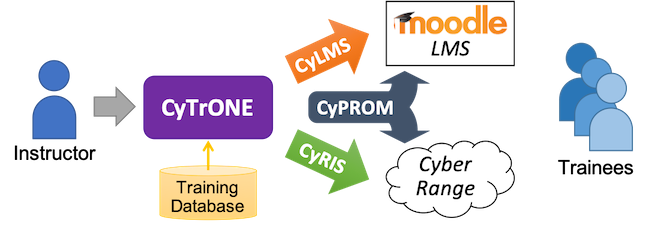
\includegraphics[width=0.92\linewidth,height=0.7\textheight,keepaspectratio]{src/images/cytrone-architecture.png}
  \caption{Cytrone Architecture}
  \label{fig:cytrone-architecture}
\end{figure}


\begin{itemize}
\tightlist
\item
  \textbf{CyLMS}: si occupa d icaricare il contenuto per il training su
  un Learning Management System come \textbf{Moodle}
\item
  \textbf{CyRIS} (Cyber Range Instantiation System): si occupa di
  istanziare l'ambiente di training su cui gli studenti possono condurre
  opportuni test per avanzare nel training.
\item
  \textbf{CyPROM}: si occupa di tracciare l'avanzamento controllando LMS
  ed il Cyber Range.
\end{itemize}

CyTrONE gestisce tre tipi di training\footnote{\label{fn:ref_9}https://www.sciencedirect.com/science/article/pii/S0167404818306527}:

\begin{itemize}
\tightlist
\item
  Training \emph{Attack-oriented}: si basa sul capire come riprodurre
  attacchi a vulnerabilita note.
\item
  Training \emph{Analysis-oriented}: si concentra sull'analisi
  dell'attacco, per capire come funziona e le sue conseguenze.
\item
  Training \textbf{Defense-oriented}: si conentra sulle tecniche di
  patching delle vulnerabilita, al fine di proteggere il sistema.
\end{itemize}

Quindi l'esperienza utente si concentra sul fatto che gli studenti
possono eseguire un training e visualizzare le risorse associate sul
Moodle ed al tempo stesso accedere al Cyber Range associato.

CyTrONE si applica bene facendo le seguenti assunzioni:

\begin{quote}
\begin{enumerate}
\def\labelenumi{\arabic{enumi})}
\tightlist
\item
  \emph{L'obiettivo di ciascuna attività di formazione può essere
  formulato come un problema, che può dipendere o meno da altri problemi
  della stessa lezione (es: trova l'indirizzo IP, trova la flag);}
  \footref{fn:ref_9}
\end{enumerate}
\end{quote}

\begin{quote}
\begin{enumerate}
\def\labelenumi{\arabic{enumi})}
\setcounter{enumi}{1}
\tightlist
\item
  \emph{Il sistema è in grado di stabilire automaticamente se il
  partecipante abbia risolto il problema, confrontando la risposta
  fornita con un valore noto} \footref{fn:ref_9}
\end{enumerate}
\end{quote}

L'architettura di CyTrONE e' supportata da un \emph{Training Database},
che si occupa di tenere in memoria le informazioni per i vari training,
che vengono caricate su CyTrONE da una figura identificata come
\emph{Training Coordinator}.Le informazioni mantenute nel database sono
per esempio: il training content, file e programmi, macchine virtuali,
ecc\ldots{} \footref{fn:ref_9}

CyTrONE utilizza un file YAML per definire il contenuto di un training:

\begin{figure}[htbp]
  \centering
  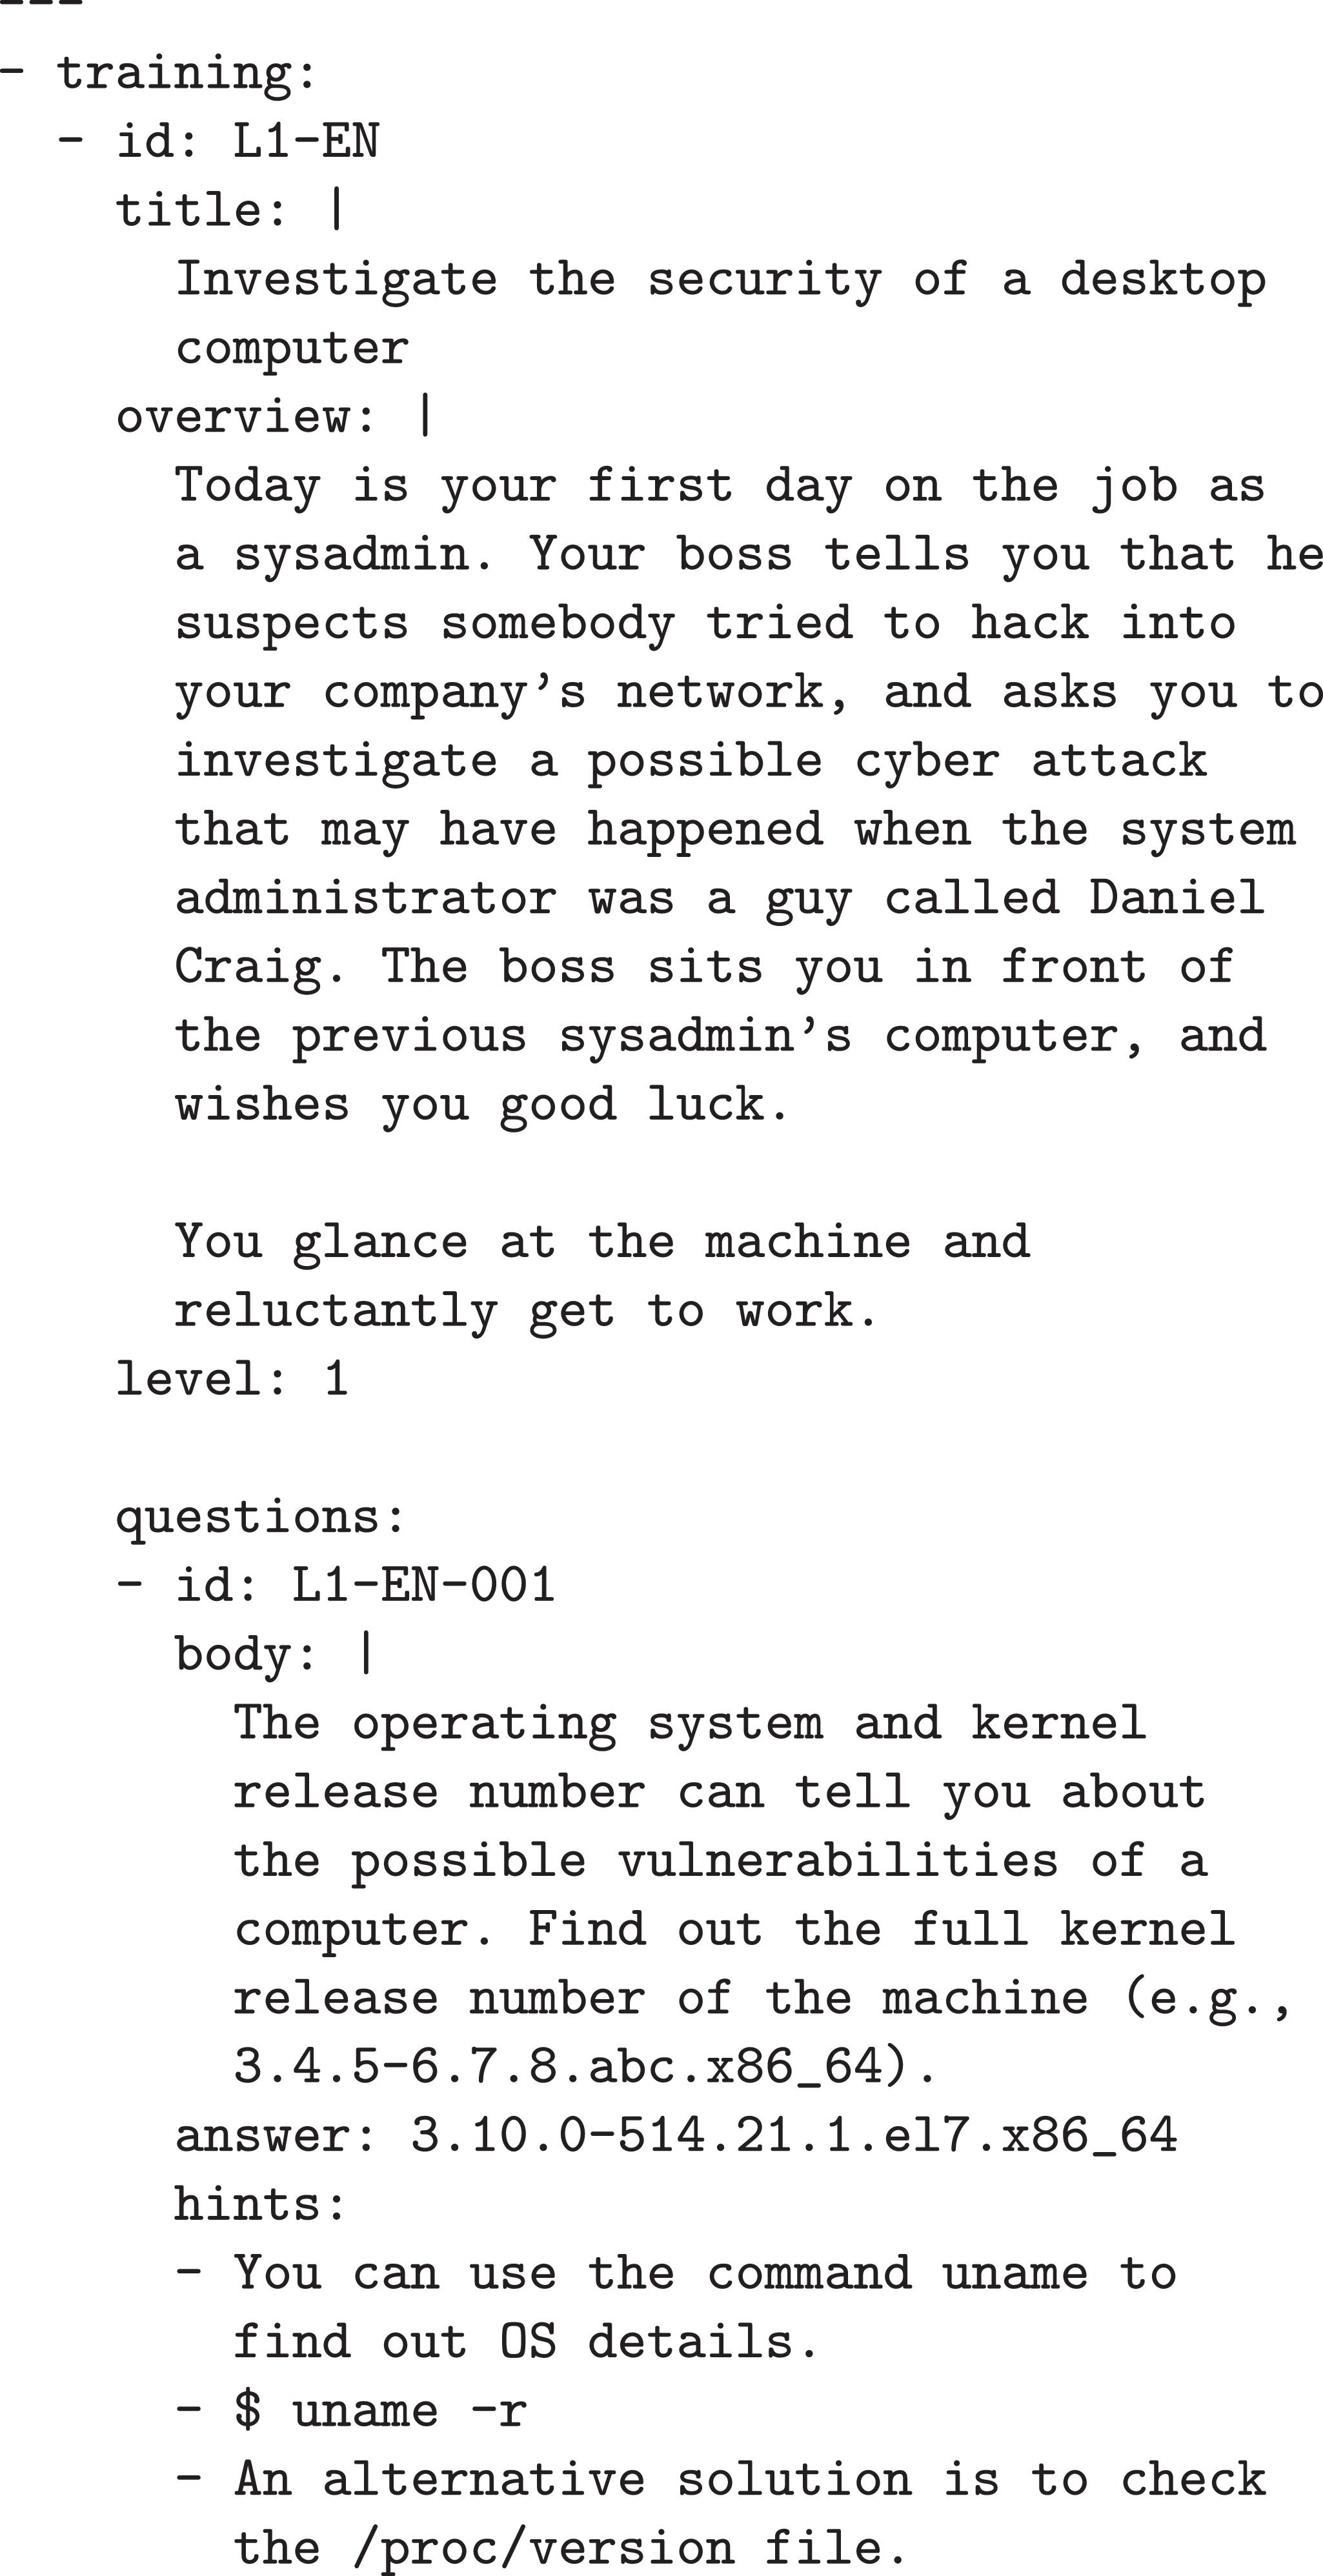
\includegraphics[width=0.92\linewidth,height=0.7\textheight,keepaspectratio]{src/images/cytrone-training.png}
  \caption{Cytrone Training}
  \label{fig:cytrone-training}
\end{figure}


E similmente, si usa un file YAML per definire la specifica del Cyber
Range:

\begin{figure}[htbp]
  \centering
  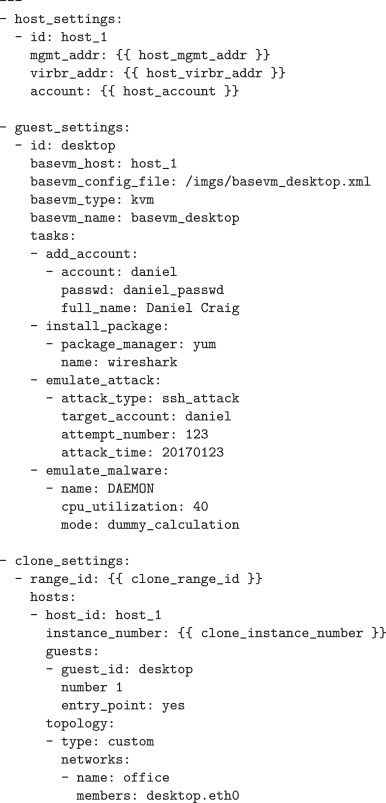
\includegraphics[width=0.92\linewidth,height=0.7\textheight,keepaspectratio]{src/images/cytrone-cyberrange.png}
  \caption{Cytrone Cyberrange}
  \label{fig:cytrone-cyberrange}
\end{figure}


A partire dalla configurazione YAML del Cyber Range, il sotto-sistema
CyRIS si occupa di istanziarlo. Successivamente, in caso di un training
\textbf{Defense-oriented} l'utente richiede l'attacco associato alla
vulnearbilita all'interno del sistema e ne viene registrato l'esisto.

Tutta via, sebbene il sistema sia ben ingegnerizzato soffre di alcuni
problemi:

\begin{enumerate}
\def\labelenumi{\arabic{enumi}.}
\tightlist
\item
  Il deploy delle vulnerabilita avviene su macchine virtuali, che
  possono costituire un alto overhead in termini di risorse, ed tempi di
  approvvigionamento lunghi per l'infrastruttura.
\item
  Il payload viene inviato remotamente dal
  \passthrough{\lstinline!cyberattack controller!} (che non fa altro che
  eseguire \passthrough{\lstinline!Metasploit!}). Tutta via il traffico
  di rete puo' essere intercettato dallo studente, ottenendo cosi
  suggerimenti per la soluzione.
\item
  L'esecuzione del payload puo scatenare la produzione di file log
  accessibili allo studente.
\item
  L'esecuzione del payload potrebbe mandare in crash il sistema del
  partecipante.
\item
  Necessita di un LMS (per design) per tenere traccia del training
  progress.
\end{enumerate}

\subsection{Valutazione delle Performance di
CyTrONE}\label{valutazione-delle-performance-di-cytrone}

Le performance di CyTrONE per il deploy dell'infrastruttura sono state
valutate usando il testbed StarBED \footnote{\label{fn:ref_10}https://www.sciencedirect.com/science/article/pii/S0167404818306527\#bib0015},
usando 30 host fisici e 600 macchine virtuali. Gli host fisici usati per
misurare le performance sono dei \emph{server rack Cisco UCS C200 M2 con
Intel Xeon E5504 2.0 GHz a 4 core e 72 GB di memoria}

Sono stati valutati 2 scenari:

\begin{itemize}
\tightlist
\item
  \emph{Level 1}: un training base che include tra gli argomenti: log,
  configurazioni di sistema, sniffing della rete e scansione delle
  vulnerabilita. Richiede un'unica macchina Virtuale per fare il deploy
  dello scenario
\item
  \emph{Level 2}: un training di difficolta media su topic come il
  network discovery, penetration testing e password cracking. Richiede
  due macchine virtuali per il deploy dello scenario.
\end{itemize}

Il processo di deploy del training, per una sola macchina virtuale, in
CyTrONE avviene in 3 fasi distinte:

\begin{enumerate}
\def\labelenumi{\arabic{enumi}.}
\tightlist
\item
  \textbf{Preparazione}: Su un nodo denominato \emph{master} viene
  configurata (per esempio, accesso tramite SSH) ed avviata la macchina
  virtuale. \(T_p\) descrive il suo tempo di esecuzione
\item
  \textbf{Installazione}: Sulla macchina nel nodo master, vengono
  installati contenuti aggiuntivi necessari per il traninig, sulla
  macchina virtuale target. \(T_i\) descrive il suo tempo di esecuzione.
\item
  \textbf{Clonazione}: Copia tramite
  \passthrough{\lstinline!parallel-scp!} dell'immagine della macchina
  sui vari nodi della rete, garantendo al tempo stesso che password e
  credenziali siano distinte per ogni immagine. \(T_c\) descrive il suo
  tempo di esecuzione
\end{enumerate}

\begin{quote}
E' dunque importante notare che per il \emph{Level 1}, bisogna clonare
con \passthrough{\lstinline!parallel-scp!} una sola immagine per nodo,
mentre per il \emph{Level 2} bisogna clonare 2 immagini per nodo.
\end{quote}

Sia \(T = T_p + T_i + T_c\), il grafico descrive come si comporta \(T\)
al variare del numero di host su cui fare il deploy delle macchine.

\begin{figure}[htbp]
  \centering
  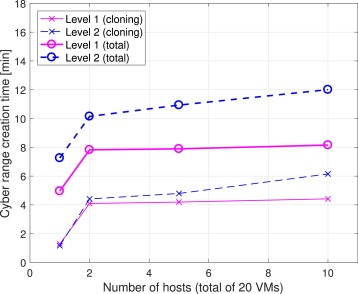
\includegraphics[width=0.92\linewidth,height=0.7\textheight,keepaspectratio]{src/images/cytrone-performance.png}
  \caption{Cytrone Performance}
  \label{fig:cytrone-performance}
\end{figure}


\begin{itemize}
\tightlist
\item
  Nei casi dove abbiamo solo 1 host, allora non c'e' bisogno di clonare
  l'immagine, basta solo un host che esegue le 20 macchine virtuali,
  ossia il master. Dunque il tempo di clonazione e' sotto i \emph{due
  minuti}, mentre \(T\) per lo scenario \emph{Level 2} si attesta sotto
  gli 8 minuti.
\item
  All'aumentare del numero \(n\) degli host, con il bisogno di clonare
  le macchine su piu nodi, il tempo di approvvigionamento totale tende a
  peggiorare, poiche bisogna trasferire l'immagine su piu nodi, sebbene
  ogni nodo gestisca solo \(20/n\) macchine virtuali.
\end{itemize}

Invece, per gli esperimenti su larga scala dove si vuole effettuare il
deploy di 20 macchine per ogni host su centinaia di host il tempo \(T\)
peggiora esponenzialmente. Nella figura sborgz viene analizzato al
variare di del numero di host fino a 600 cosa succede se ogni nodo deve
eseguire 20 macchine, con 20 immagini differenti.

\begin{figure}[htbp]
  \centering
  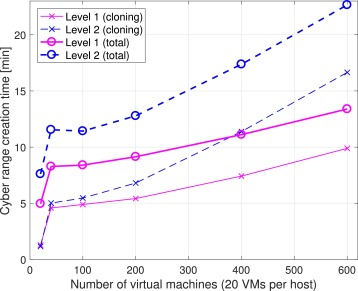
\includegraphics[width=0.92\linewidth,height=0.7\textheight,keepaspectratio]{src/images/cytrone-largescaleperformance.png}
  \caption{Cytrone Largescaleperformance}
  \label{fig:cytrone-largescaleperformance}
\end{figure}


Le differenze tra CyTrONE e Blueagent sono elencate nella seguente
tabella:

\begin{longtable}[]{@{}
  >{\raggedright\arraybackslash}p{(\linewidth - 4\tabcolsep) * \real{0.3333}}
  >{\raggedright\arraybackslash}p{(\linewidth - 4\tabcolsep) * \real{0.3333}}
  >{\raggedright\arraybackslash}p{(\linewidth - 4\tabcolsep) * \real{0.3333}}@{}}
\toprule\noalign{}
\begin{minipage}[b]{\linewidth}\raggedright
Caratteristica
\end{minipage} & \begin{minipage}[b]{\linewidth}\raggedright
CyTrONE
\end{minipage} & \begin{minipage}[b]{\linewidth}\raggedright
BlueAgent
\end{minipage} \\
\midrule\noalign{}
\endhead
\bottomrule\noalign{}
\endlastfoot
\textbf{Virtualizzazione} & Macchine Virtuali & Container di sistema \\
\textbf{Infrastruttura} & Cluster distribuito su larga scala (es:
\emph{StarBED}) & Singolo nodo host \\
\textbf{Isolamento e Verifica} & Il controller invia exploit via rete &
Exploit inviati in una rete separata inaccessibile al giocatore \\
\textbf{Rete} & Reti virtuali KVM & Linux Bridge per L2, SDN, WireGuard
per L3 \\
\textbf{Scopo Principale} & Formazione didattica guidata con Moodle e
verifiche statiche sulle macchine & Cyber Range compatto per
competizioni di Difesa \\
\end{longtable}
